Sei $k$ ein Kreis mit Mittelpunkt $O$. Sei $AB$ eine Sehne dieses Kreises mit Mittelpunkt $M \neq O$. Die Tangenten von $k$ an $A$ und $B$ schneiden sich in $T$. Die Gerade $l$ geht durch $T$ und schneidet $k$ in $C$ und $D$, mit $CT < DT$ und $BC = BM$.

Beweise, dass der Umkreismittelpunkt des Dreiecks $ADM$ die Spiegelung von $O$ an der Geraden $AD$ ist.

\textbf{Lösung}: Für diese Aufgabe gibt es zwei verschiedene Ansätze um die Aufgabe zu lösen. Die erste Lösung verwendet einen andere Definition der Punkte und Potenzlinien, die zweite Lösung verwendet den Symmedian, welchen wir ab nächsten Jahr auch in der Selektion behandeln. 

\textbf{Solution 1 (français)} On souhaite prouver que la réflexion de $C$ par rapport à la droite $OM$ est sur la droite $DM$. Appelons ce point $C'$. Il n'y a malheureusement pas de manière simple de prouver un tel résultat.
Pour cette raison nous introduisons les points $E$ et $E'$. $E$ est la seconde intersection de la droite $C'M$ avec le cercle $k$ et $E'$ est la seconde intersection de la droite $CM$ avec le cercle $k$. Nous voulons prouver que les droites $CE$, $OM$ ainsi que la tangente à $k$ au point $B$ se coupent en un point. Si cette propriété est vérifiée, il s'ensuit que la droite $CE$ est la droite $CD$ et donc $D = E$.

\begin{figure}[h]
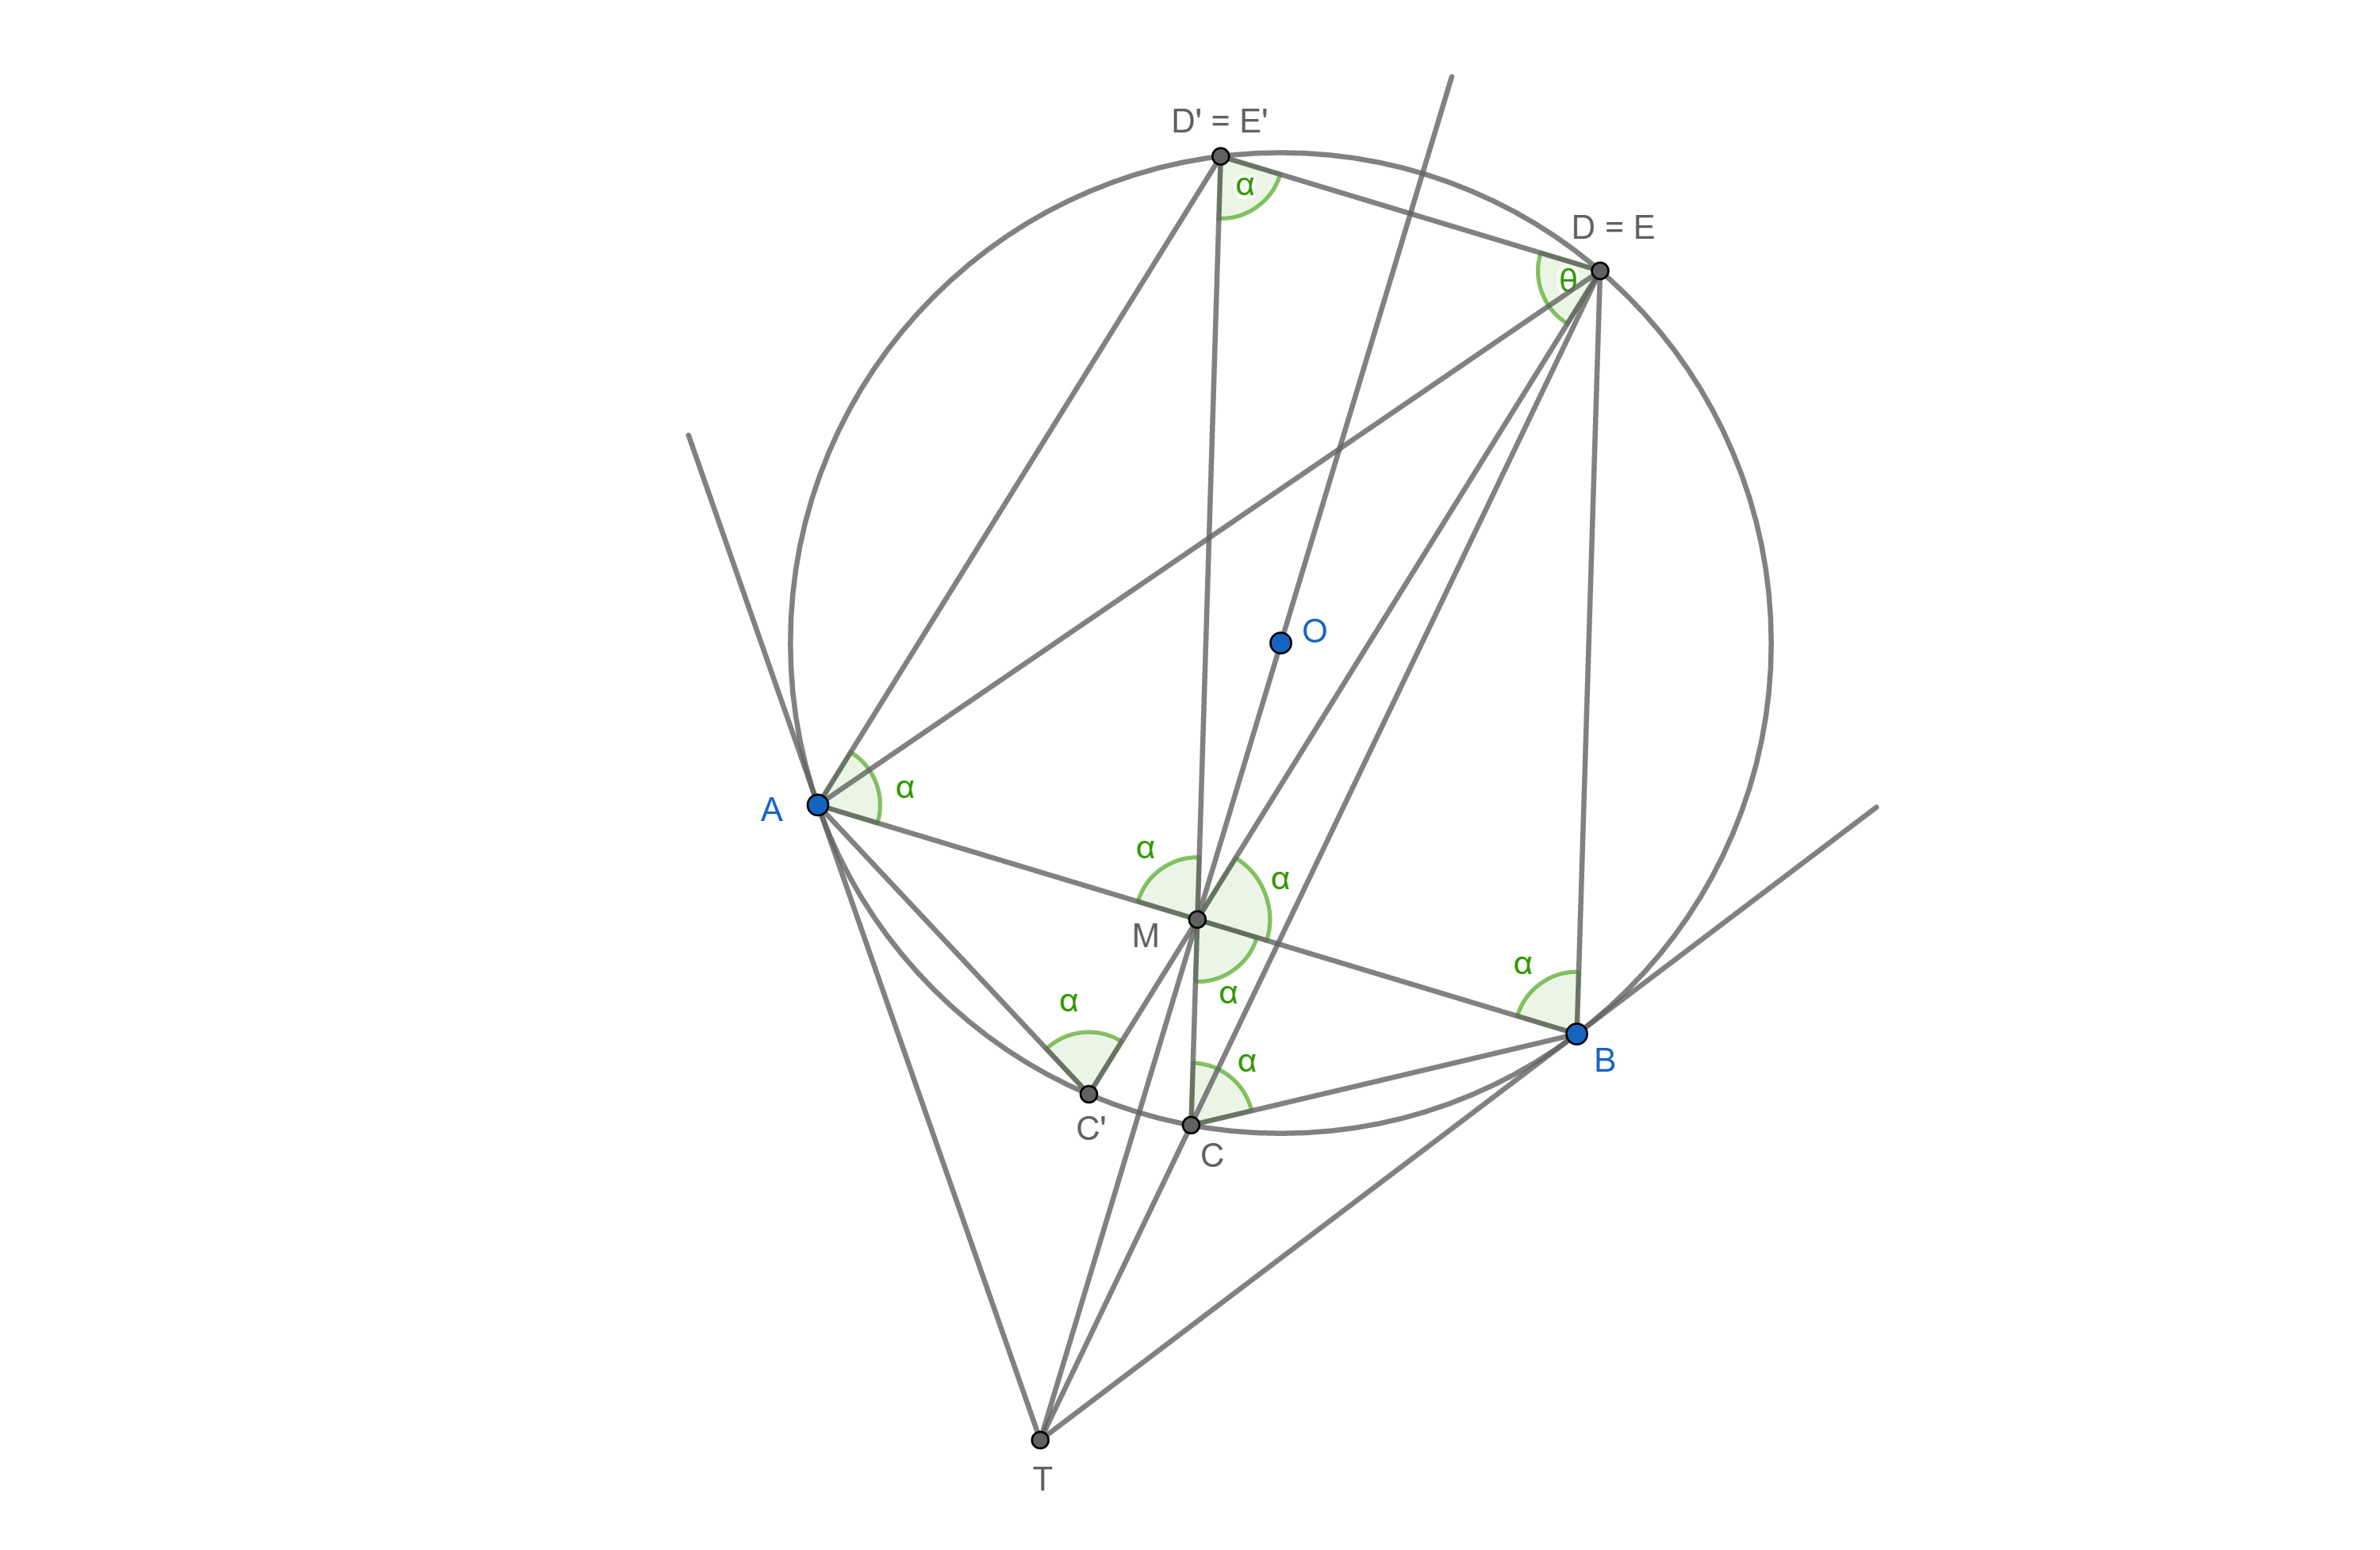
\includegraphics[width = \textwidth]{2020/selektion/musterloesung/solutions/s3_bis.png}
\caption{Lösung zur Aufgabe S3}
\end{figure}

Soit $\alpha = \angle BCM$. Puisque $BC = BM = AM = AC'$ nous avons $\angle CMB = \angle AMC' = \angle AC'M = \angle AC'E = \angle BCE' = \alpha$. De plus nous avons également $\angle ABE = \angle AC'E = \alpha$ et $\angle BAE' = \angle BCE' = \alpha$. Il s'ensuit que $\angle CBE = 180^{\circ} - 2\alpha + \alpha  = 180^{\circ} - \alpha$ et ainsi $\angle COE = 2\alpha = \angle CME$. Par conséquent $CMOE$ est un quadrilatère inscrit. Soit $N$ le milieu du segment $OB$. Le point $T$ appartient à la ligne de puissance du cercle de centre $N$ passant par $B, M, O$ et du cercle $k$ ainsi qu'à la ligne de puissance de ce même cercle et du cercle circonscrit à $CMOB$, dont $T$ appartient à la ligne de puissance du cercle circonscrit à $CMOB$ et du cercle $k$, qui est la droite $CE$. Par conséquent $E, C, T$ sont alignés et donc $D = E$. On prouve de la même manière que $E' = D'$, avec $D'$ la réflexion de $D$ par rapport à la droite $OM$.
Par les propriétés des réflexions $MD' = MD$. D'autre part $AD'M$ est un triangle isocèle donc on a $AD' = MD' = MD$. D'autre part $180^{\circ} - \angle AMD = \angle BMD = \alpha = \angle MAD'$ donc $AMDD'$ est un parallélogramme et puisque $O$ est le centre du cercle circonscrit à $AD'D$, la réflexion de $O$ par rapport à $AD$ est le centre du cercle circonscrit à $AMD$.

\textbf{1. Lösung (deutsch)}
Wir möchten zuerst irgendwie beweisen, dass die Spiegelung von $C$ an der Geraden $OM$ auf der Geraden $DM$ liegt. Nennen wir diesen Punkt $C'$. Allerdings gibt es keinen einfachen Weg, dies zu beweisen. 
Aus diesem Grund führen wir die Punkte $E$ und $E'$ ein. $E$ ist der zweite Schnittpunkt des Kreises $k$ mit der Geraden $C'M$ und $E'$ ist der zweite Schnittpunkt $k$ mit der Geraden $CM$. Wir möchten nun beweisen, dass die Geraden $CE$, $OM$, und die Tangente an $k$ durch $B$ sich in einem Punkt schneiden, woraus folgt dass $D = E$. 

Sei $\angle BCM = \alpha$. Wegen $BC = BM = AM = AC'$ hat man $\angle CMB = \angle AMC' = \angle AC'M = \angle AC'E = \angle BCE' = \alpha.$ 
Daraus folgt $\angle CBE = 180^\circ - \alpha$ und somit $\angle COE = 2 \alpha = \angle CME$. $CMOE$ bildet also ein Sehnenviereck. Sei $N$ der Mittelpunkt von $OB$. Die Potenzlinien des Kreises mit Mittelpunkt $N$ durch $BMO$, des Kreises durch $CMOE$ und von $k$ schneiden sich in einem Punkt, $T$. 
Also gilt $D = E$ und $D'=E'$. 
Aus $AD' = MD' = MD$ folgt, dass $\angle MD'D = DD'M = \alpha$. Somit ist $AMD'D$ ein Parallelogramm und da $O$ der Mittelpunkt des Kreises durch $ADD'$ ist, ist die Spiegelung von $O$ an $AD$ der Mittelpunkt des Kreises durch $AMD$. 

\textbf{2. Lösung}
Wegen der Eigenschaft des Symmedians folgt $\angle ADM = \angle CDB$. Ausserdem gilt $\angle MAD = \angle BAD = \angle BCD$ und $BC = AM$. Die Dreiecke $BCD$ und $MAD$ sind kongruent zueinander. 
Somit folgt, dass $R_{AMD}=R_{CBD}=OD=OB$. Aber weil $OM<OB$ ist $O$ nicht der Mittelpunkt des Kreises durch $AMD$. Die einzige Möglichkeit für einen Mittelpunkt ist somit die Spiegelung von $O$ an der Geraden $AD$. 

\textbf{Marking Scheme Lösung 1:}
\begin{itemize}
    \item 1P : Feststellen, dass man beweisen möchte $C'$, $M$ und $D$ sind auf einer Geraden, oder dass $E'$ die Spiegelung von D an $OM$ ist oder eine gleichbedeutende Aussage.
    \item 3P: Beweisen, dass der Punkt $C$ und der Schnittpunkt von $MD$ mit $k$ symmetrisch in $MO$ ist.
    \item 1P: Daraus folgern, dass $AMDD'$ ein Parallelogramm ist.
    \item 2P: Den Beweis vollenden. 
\end{itemize}
 \textbf{Marking Scheme Lösung 2:}
 \begin{itemize}
     \item 1P: Feststellen, dass $DT$ der Symmedian ist, da $T$ der Schnittpunkt der Tangenten ist.
     \item 2P: Herausfinden, dass $\angle ADM = \angle CDB$.
     \item 2P: Beweisen, dass $AMD$ und $CBD$ kongruent sind. 
     \item 2P: Den Beweis vollenden. 
 \end{itemize}
 -1P: In a partial or complete solution, insufficiently arguing that $DT$ is a symmedian (minimal requirement is either explicitly stating that the reason is that $T$ is the intersection of the tangents, or providing an unambiguous reference)






